
\section{proteins.xml, rnas.xml and dna.xml}

All these files use instances of the class \rbamacromolecules.


\subsection{RBAMacromolecules}
\label{sec:rba_macromolecules}

The outermost portion of the metabolism file is an instance of class
\rbamacromolecules, shown in Figure~\ref{fig:macromolecules}.

\begin{figure}
  \centering
  \includegraphics[scale=0.8]{figures/macromolecules}
  \caption{XML structure of macromolecule document.}
\label{fig:macromolecules}
\end{figure}

\rbamacromolecules{} has no simple attributes.
It contains exactly one instance of \textbf{ListOfComponents}
and \textbf{ListOfMacromolecules}.


\subsection{Component}
\label{sec:component}

The \component{} class is used to define the components of a \macromolecule{}
(Fig.~\ref{fig:macromolecules}).
For example, these are expected to be amino acids, vitamins and ions for
proteins.
Note that they use separate identifiers as metabolic \species.
\componentmap{}s define how they are assembled from metabolites.


\paragraph{The \textit{id} attribute}
The \textbf{id} attribute is a string defining the identifier of a component.

\paragraph{The \textit{weight} attribute}
The \textbf{weight} attribute is a real number defining the weight of a
component.
This information is essential for the density constraints.
The weight of a macromolecule is defined as the sum of the weight of its
components.
Note that units used for the weight constraint must be consistent across
files.

\paragraph{The \textit{name} and \textit{type} attributes}
The \textbf{name} and \textbf{type} attributes are string that provide
additional information about the component.
The name is a standard name of the component
(\textit{e.g.} full amino acid name).
The type can be used to distinguish components if necessary
(\textit{e.g.} in amino acids, vitamins, ions).


\subsection{Macromolecule}
\label{sec:macromolecule}

The \macromolecule{} class is used to define macromolecular species
(Fig.~\ref{fig:macromolecules}).
Its composition is given by a \textbf{ListOfComponentReferences}.

\paragraph{The \textit{id} attribute}
The \textbf{id} attribute is a string defining the identifier of
the macromolecule.

\paragraph{The \textit{compartment} attribute}
The \textbf{compartment} attribute must match the identifier of a \compartment.
It represents the compartment where the molecule is thought to be active.


\subsection{ComponentReference}
\label{sec:component_reference}

The \componentreference{} class is used to refer to a \component{}
and associate with it a stoichiometry (Fig.~\ref{fig:macromolecules}).

\paragraph{The \textit{component} attribute}
The \textbf{component} attribute must match the identifier of a \component{}
defined in the same \rbamacromolecules{} instance.

\paragraph{The \textit{stoichiometry} attribute}
The \textbf{stoichiometry} is a positive real number.
It repensents the stoichiometry of a \component{} in a given context
(typically the composition of a \macromolecule).
